% Construct a figure similar to Fig. 2.5 in the book of Kuznetsov.

\begin{figure}[H]
    \centering
    \begin{subfigure}[b]{\textwidth}
        \centering
        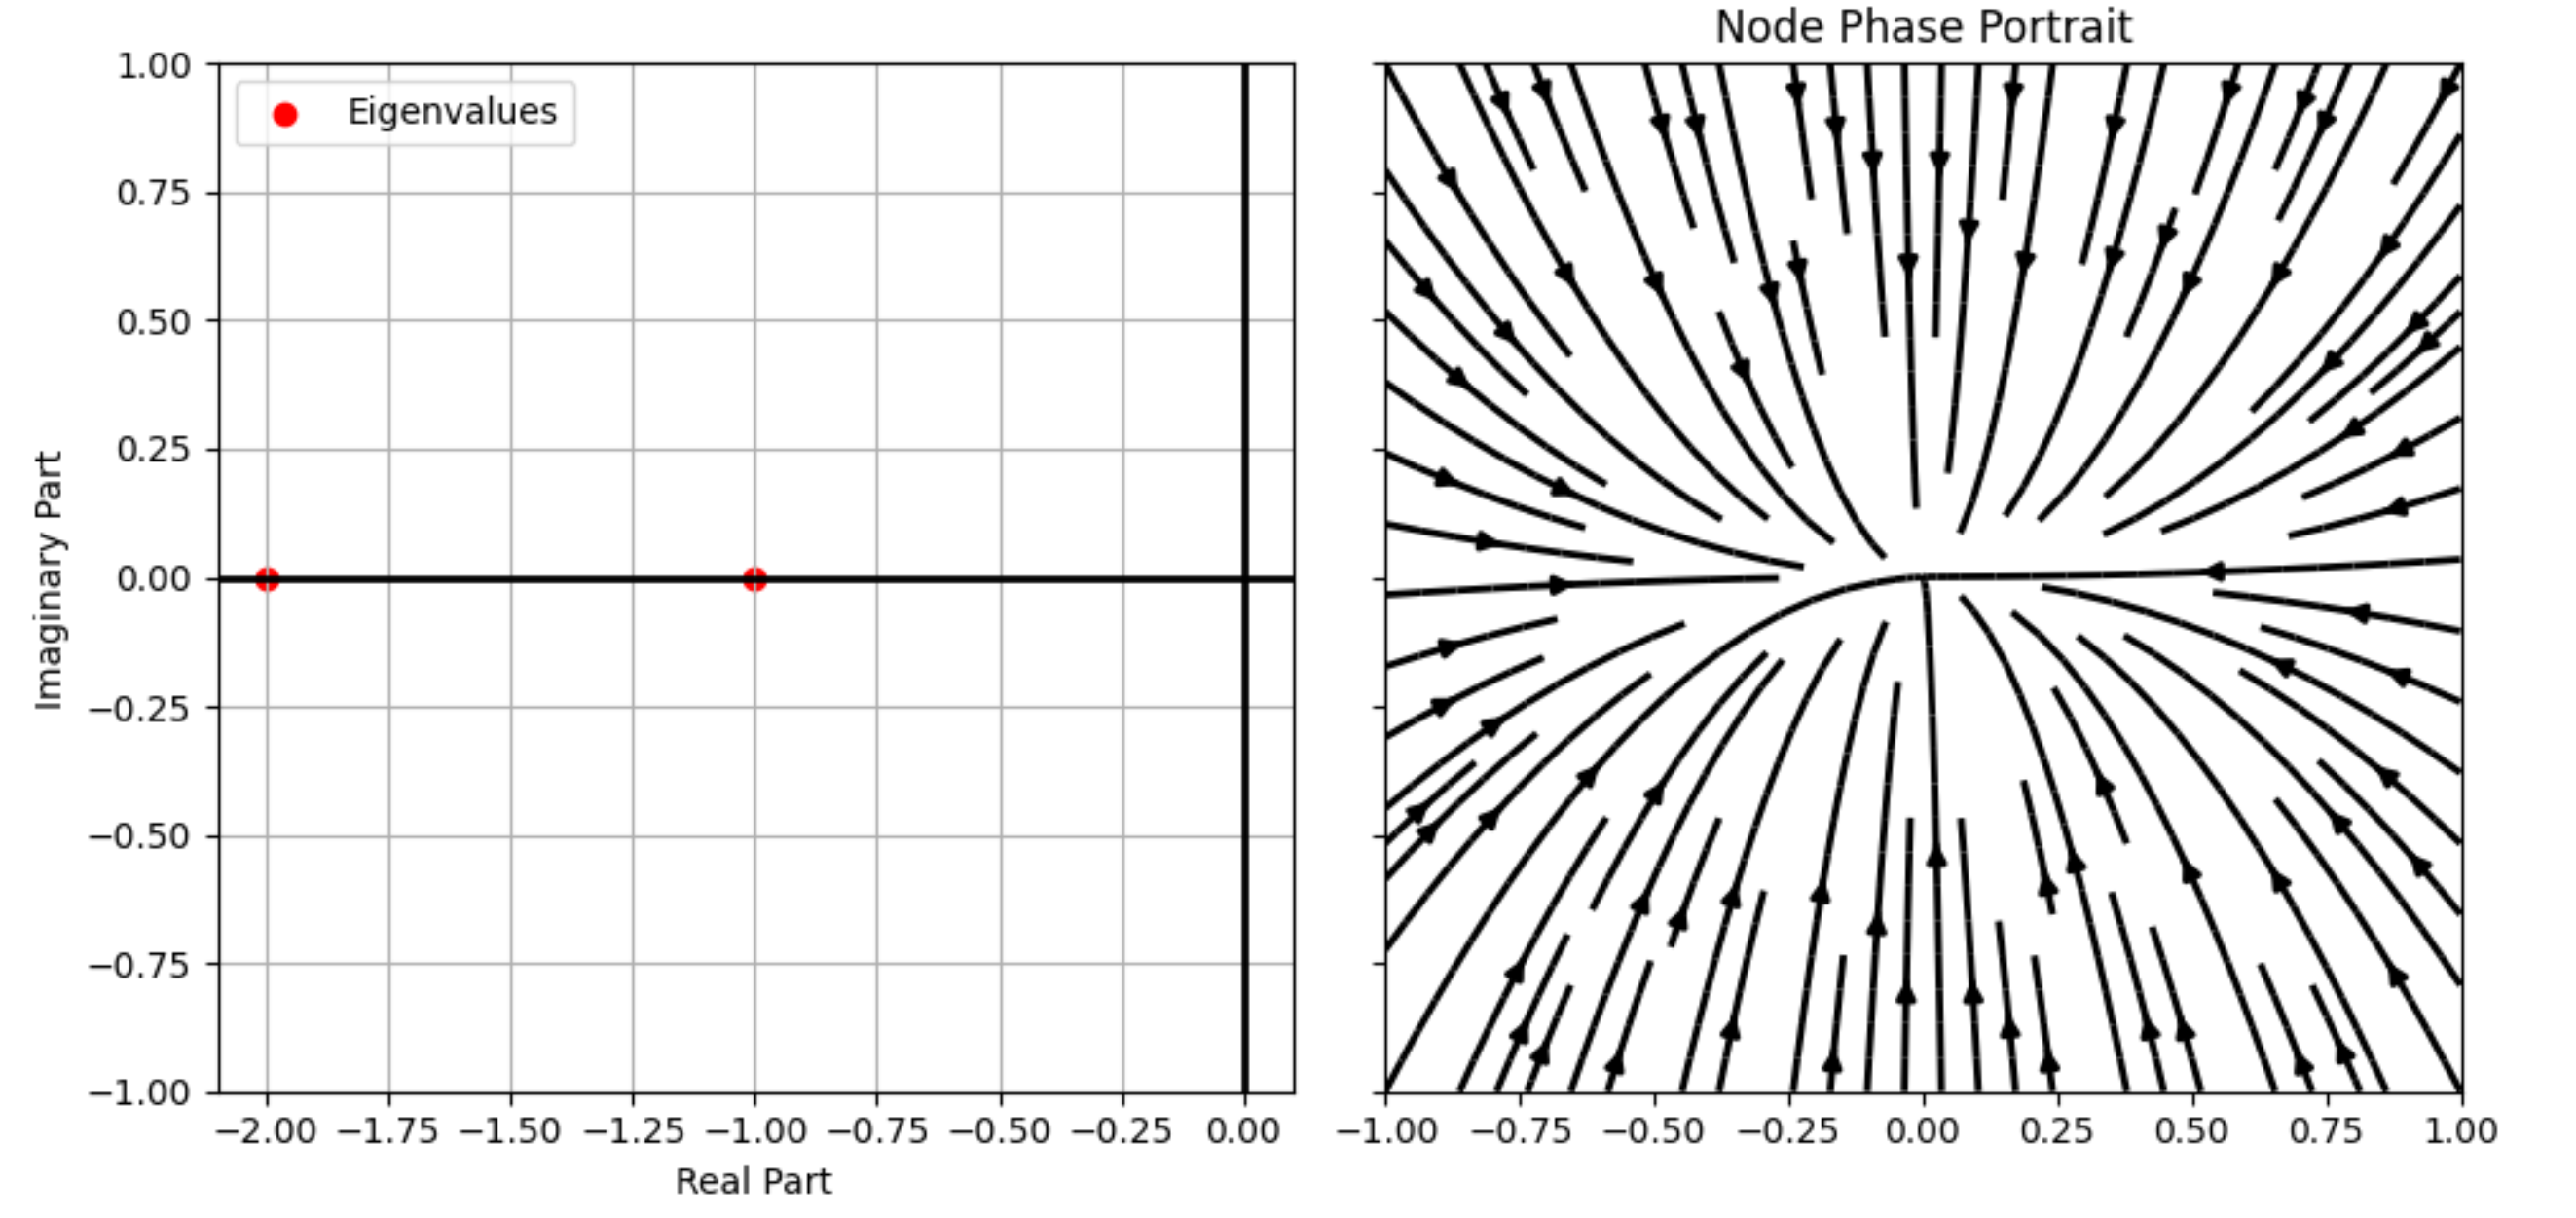
\includegraphics[width=0.8\textwidth]{images/4-1-Node.png}
    \end{subfigure}
    \begin{subfigure}[b]{\textwidth}
        \centering
        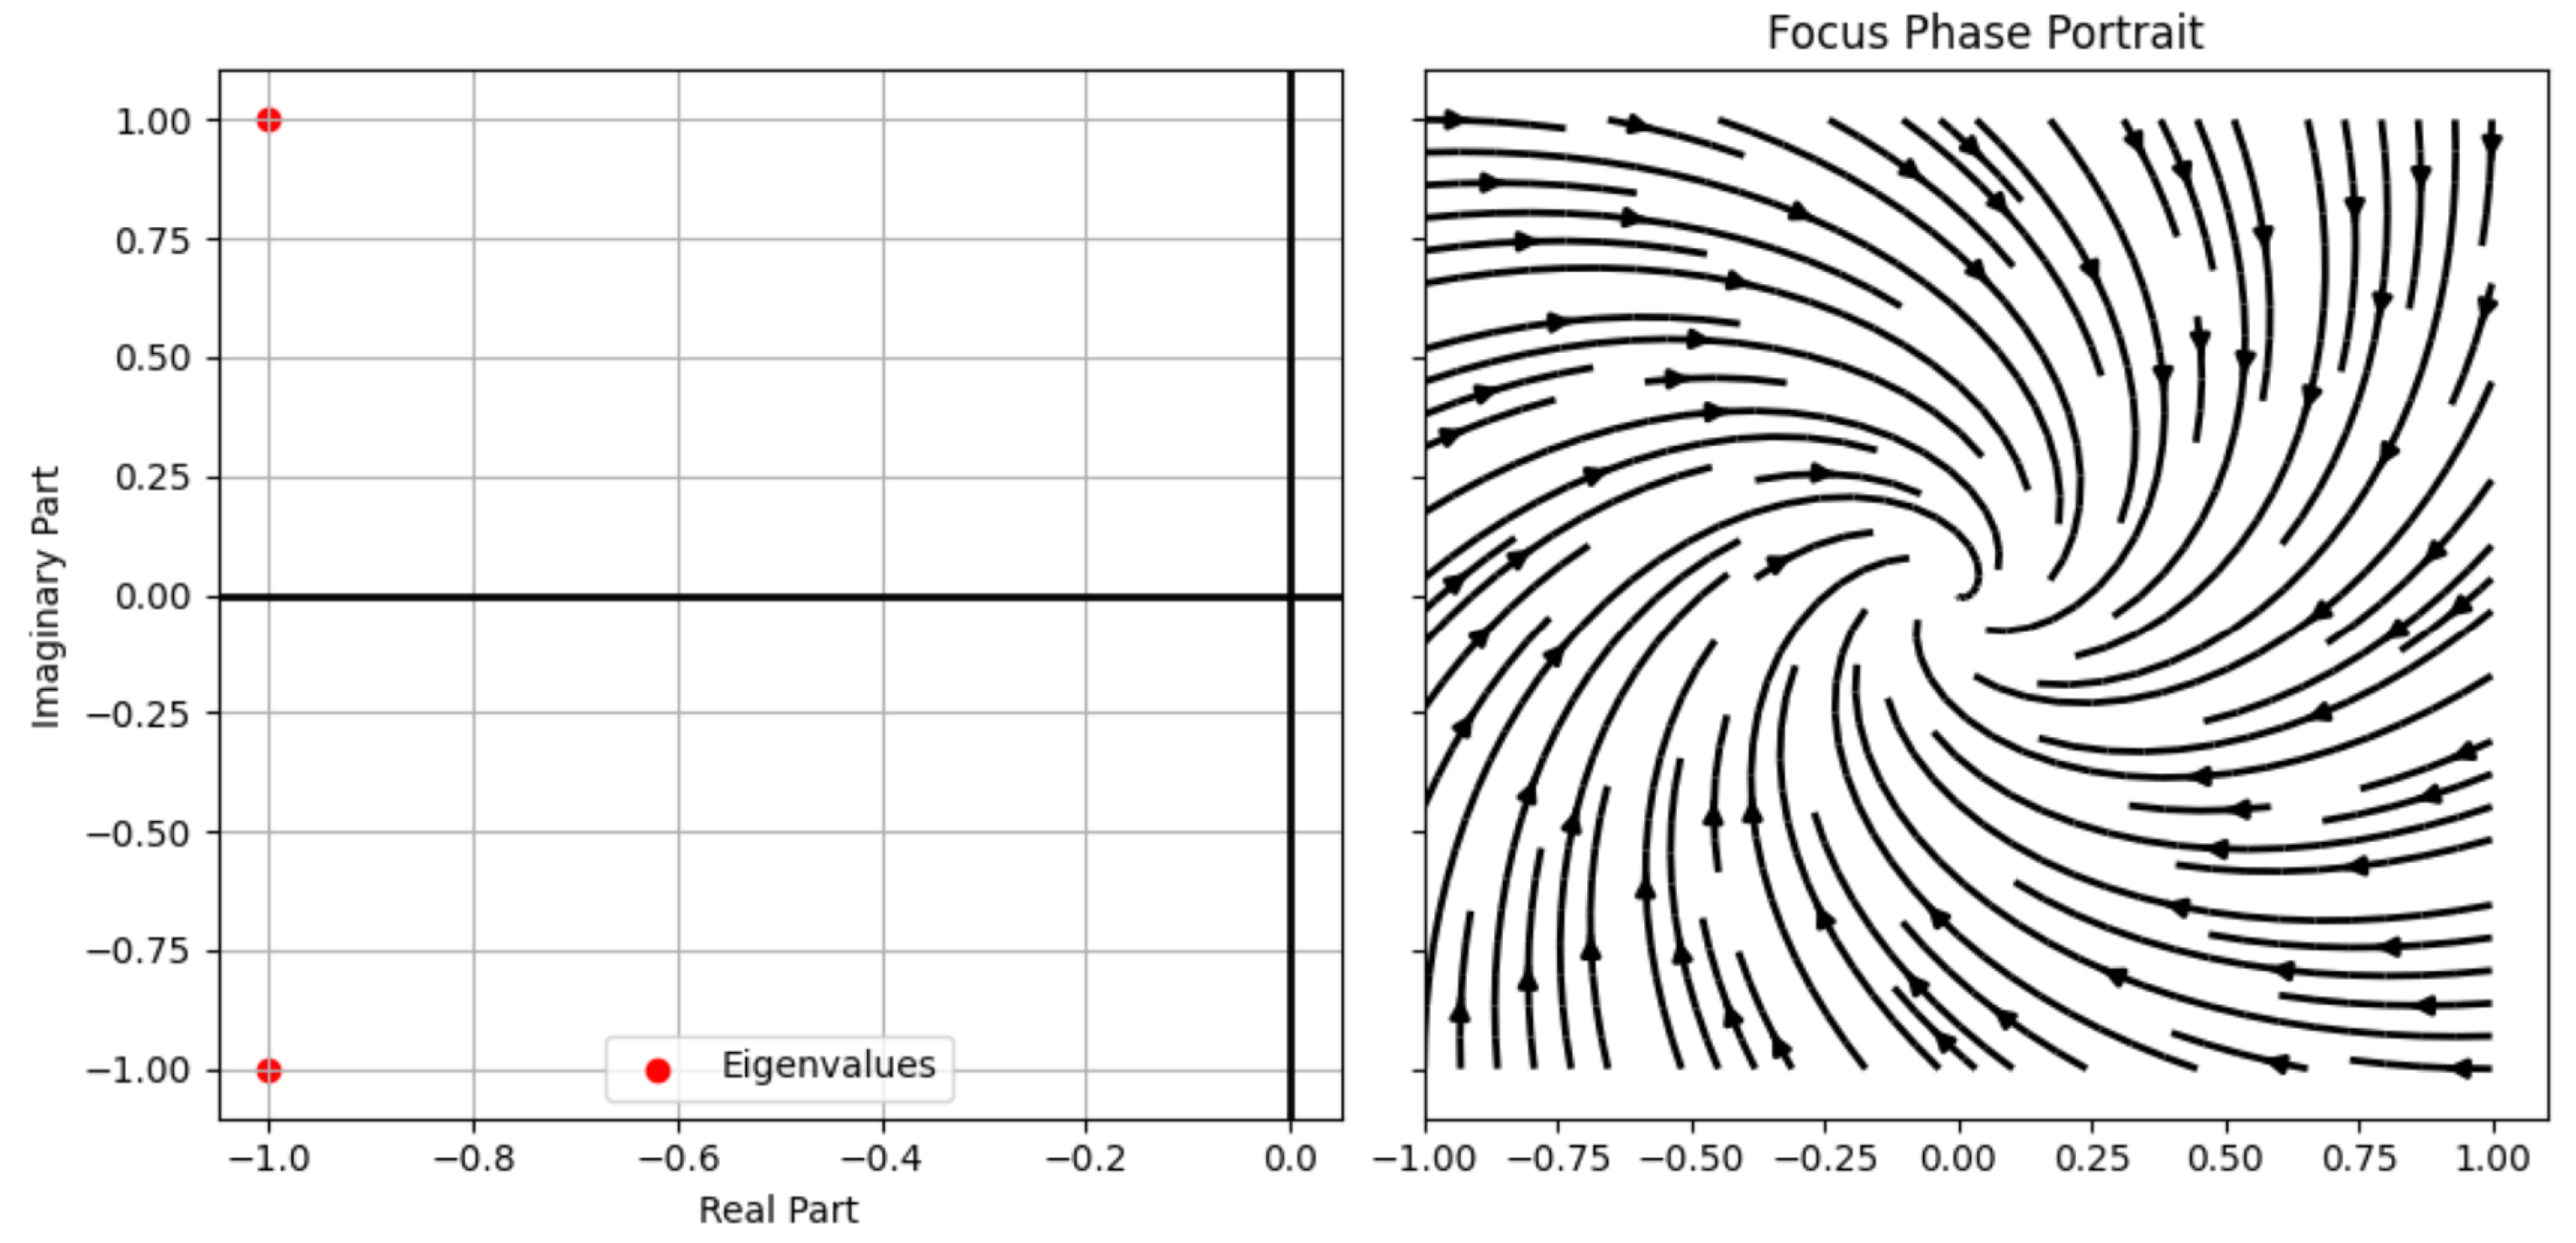
\includegraphics[width=0.8\textwidth]{images/4-1-Focus.png}
    \end{subfigure}
    \begin{subfigure}[b]{\textwidth}
        \centering
        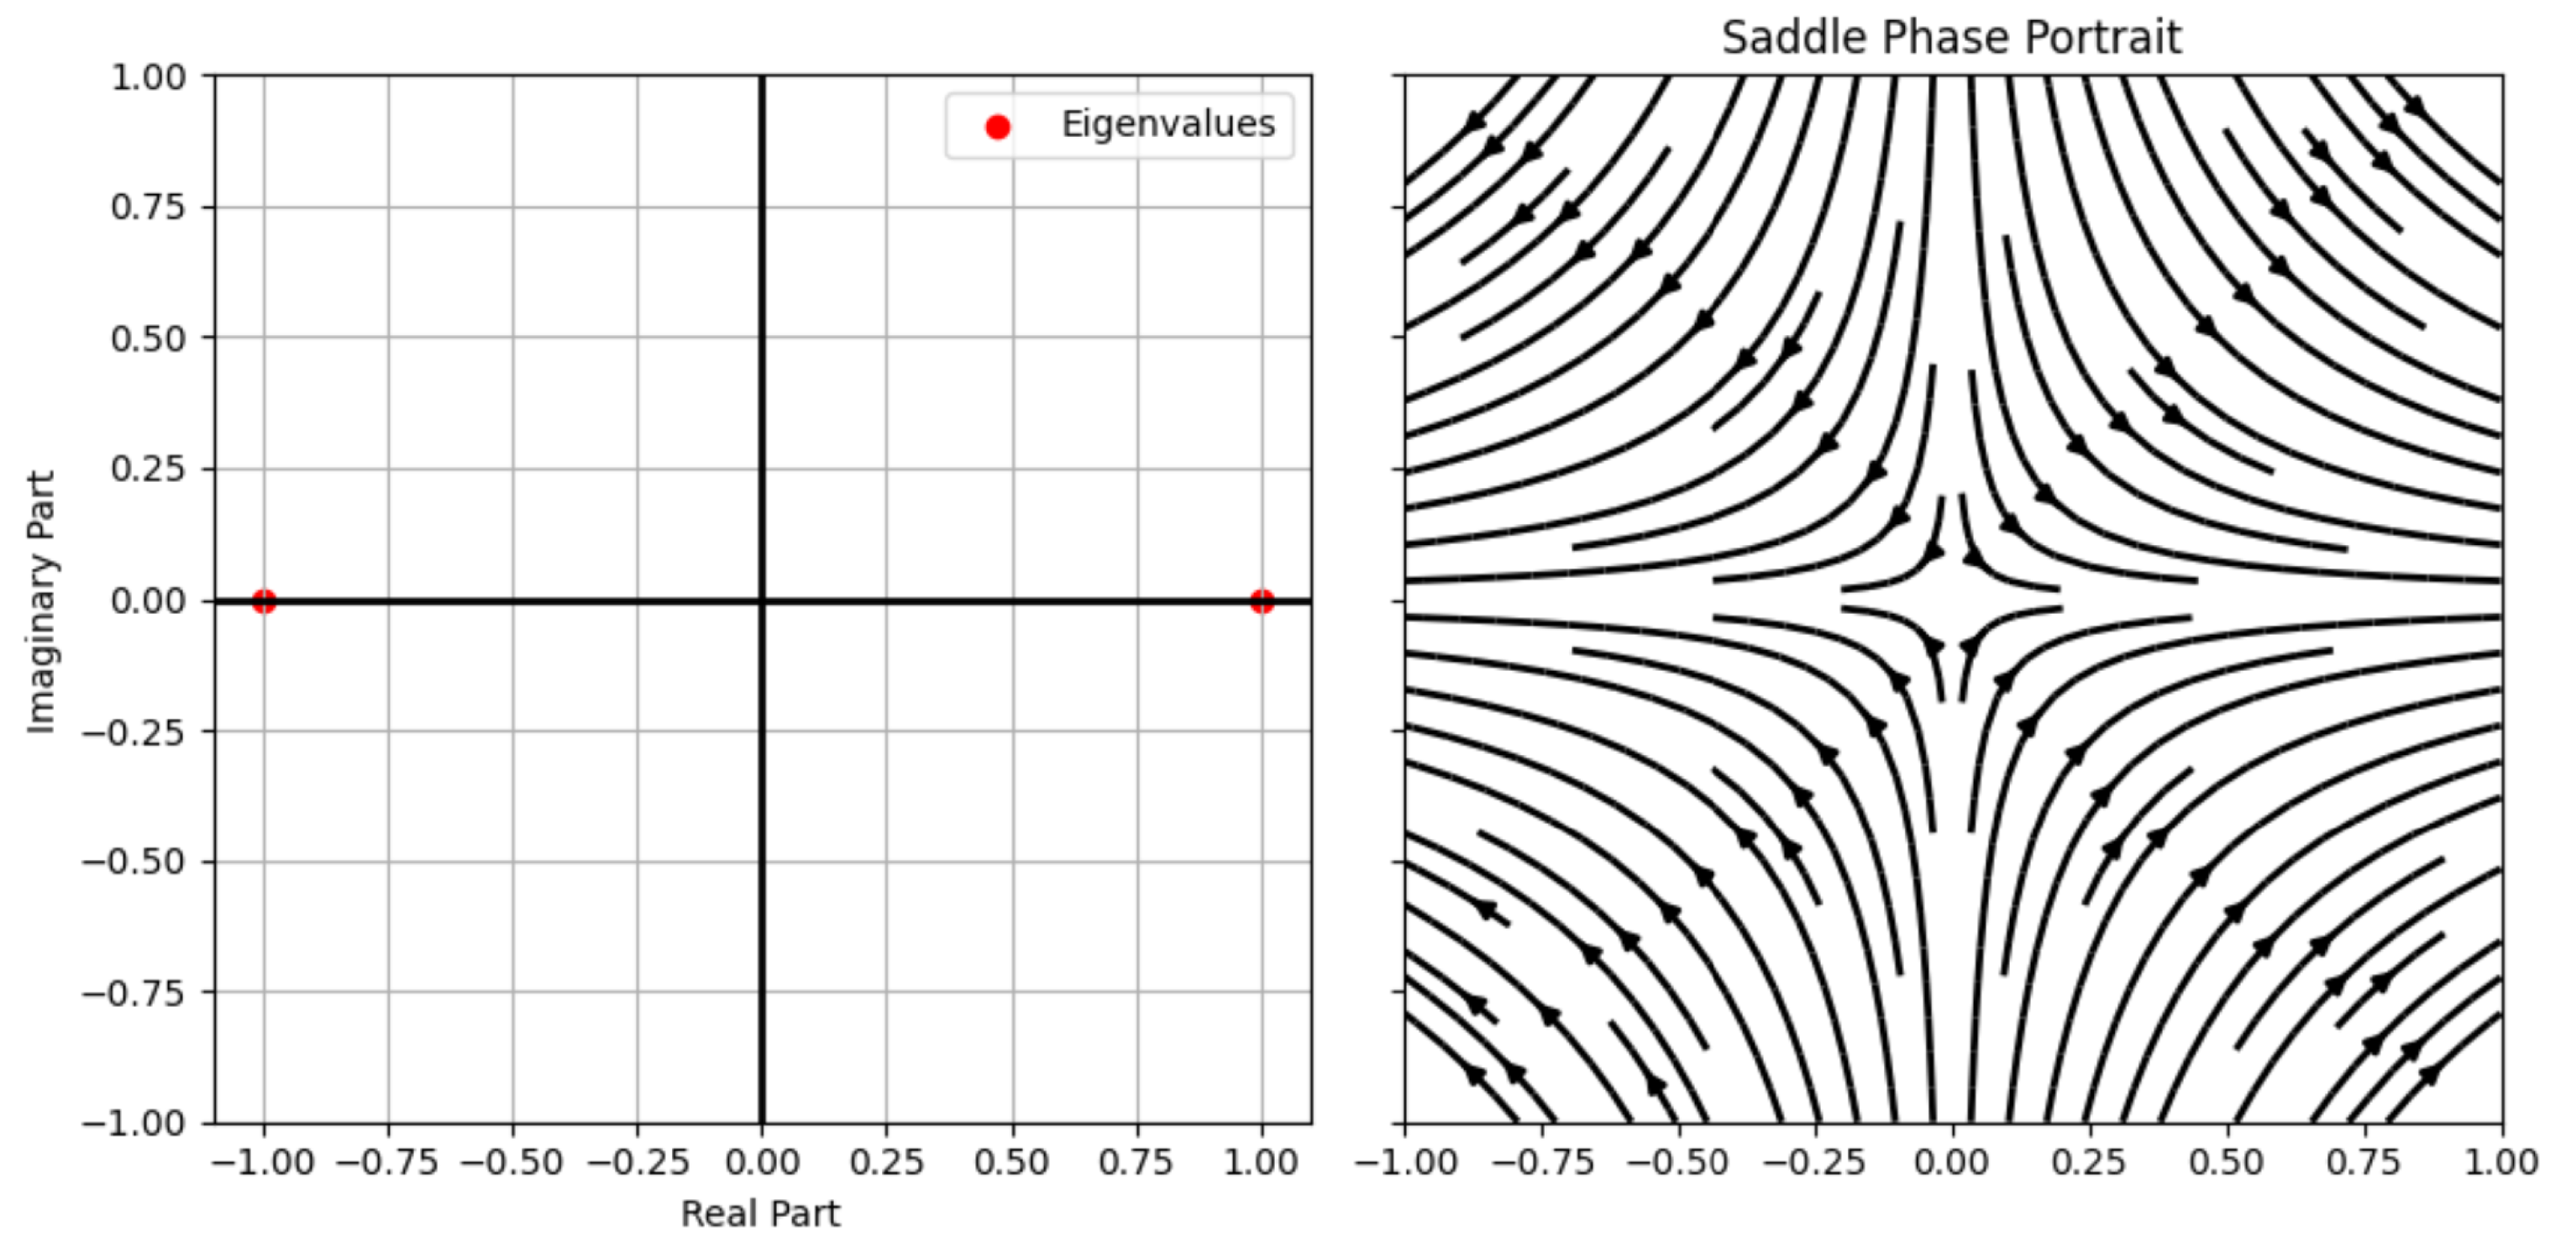
\includegraphics[width=0.8\textwidth]{images/4-1-Saddle.png}
    \end{subfigure}
    \caption{Phase portraits depending on the eigenvalues of the parametrized matrix}
    \label{fig:task1}
\end{figure}

\begin{figure}[H]\ContinuedFloat
    \centering
    \begin{subfigure}[b]{\textwidth}
        \centering
        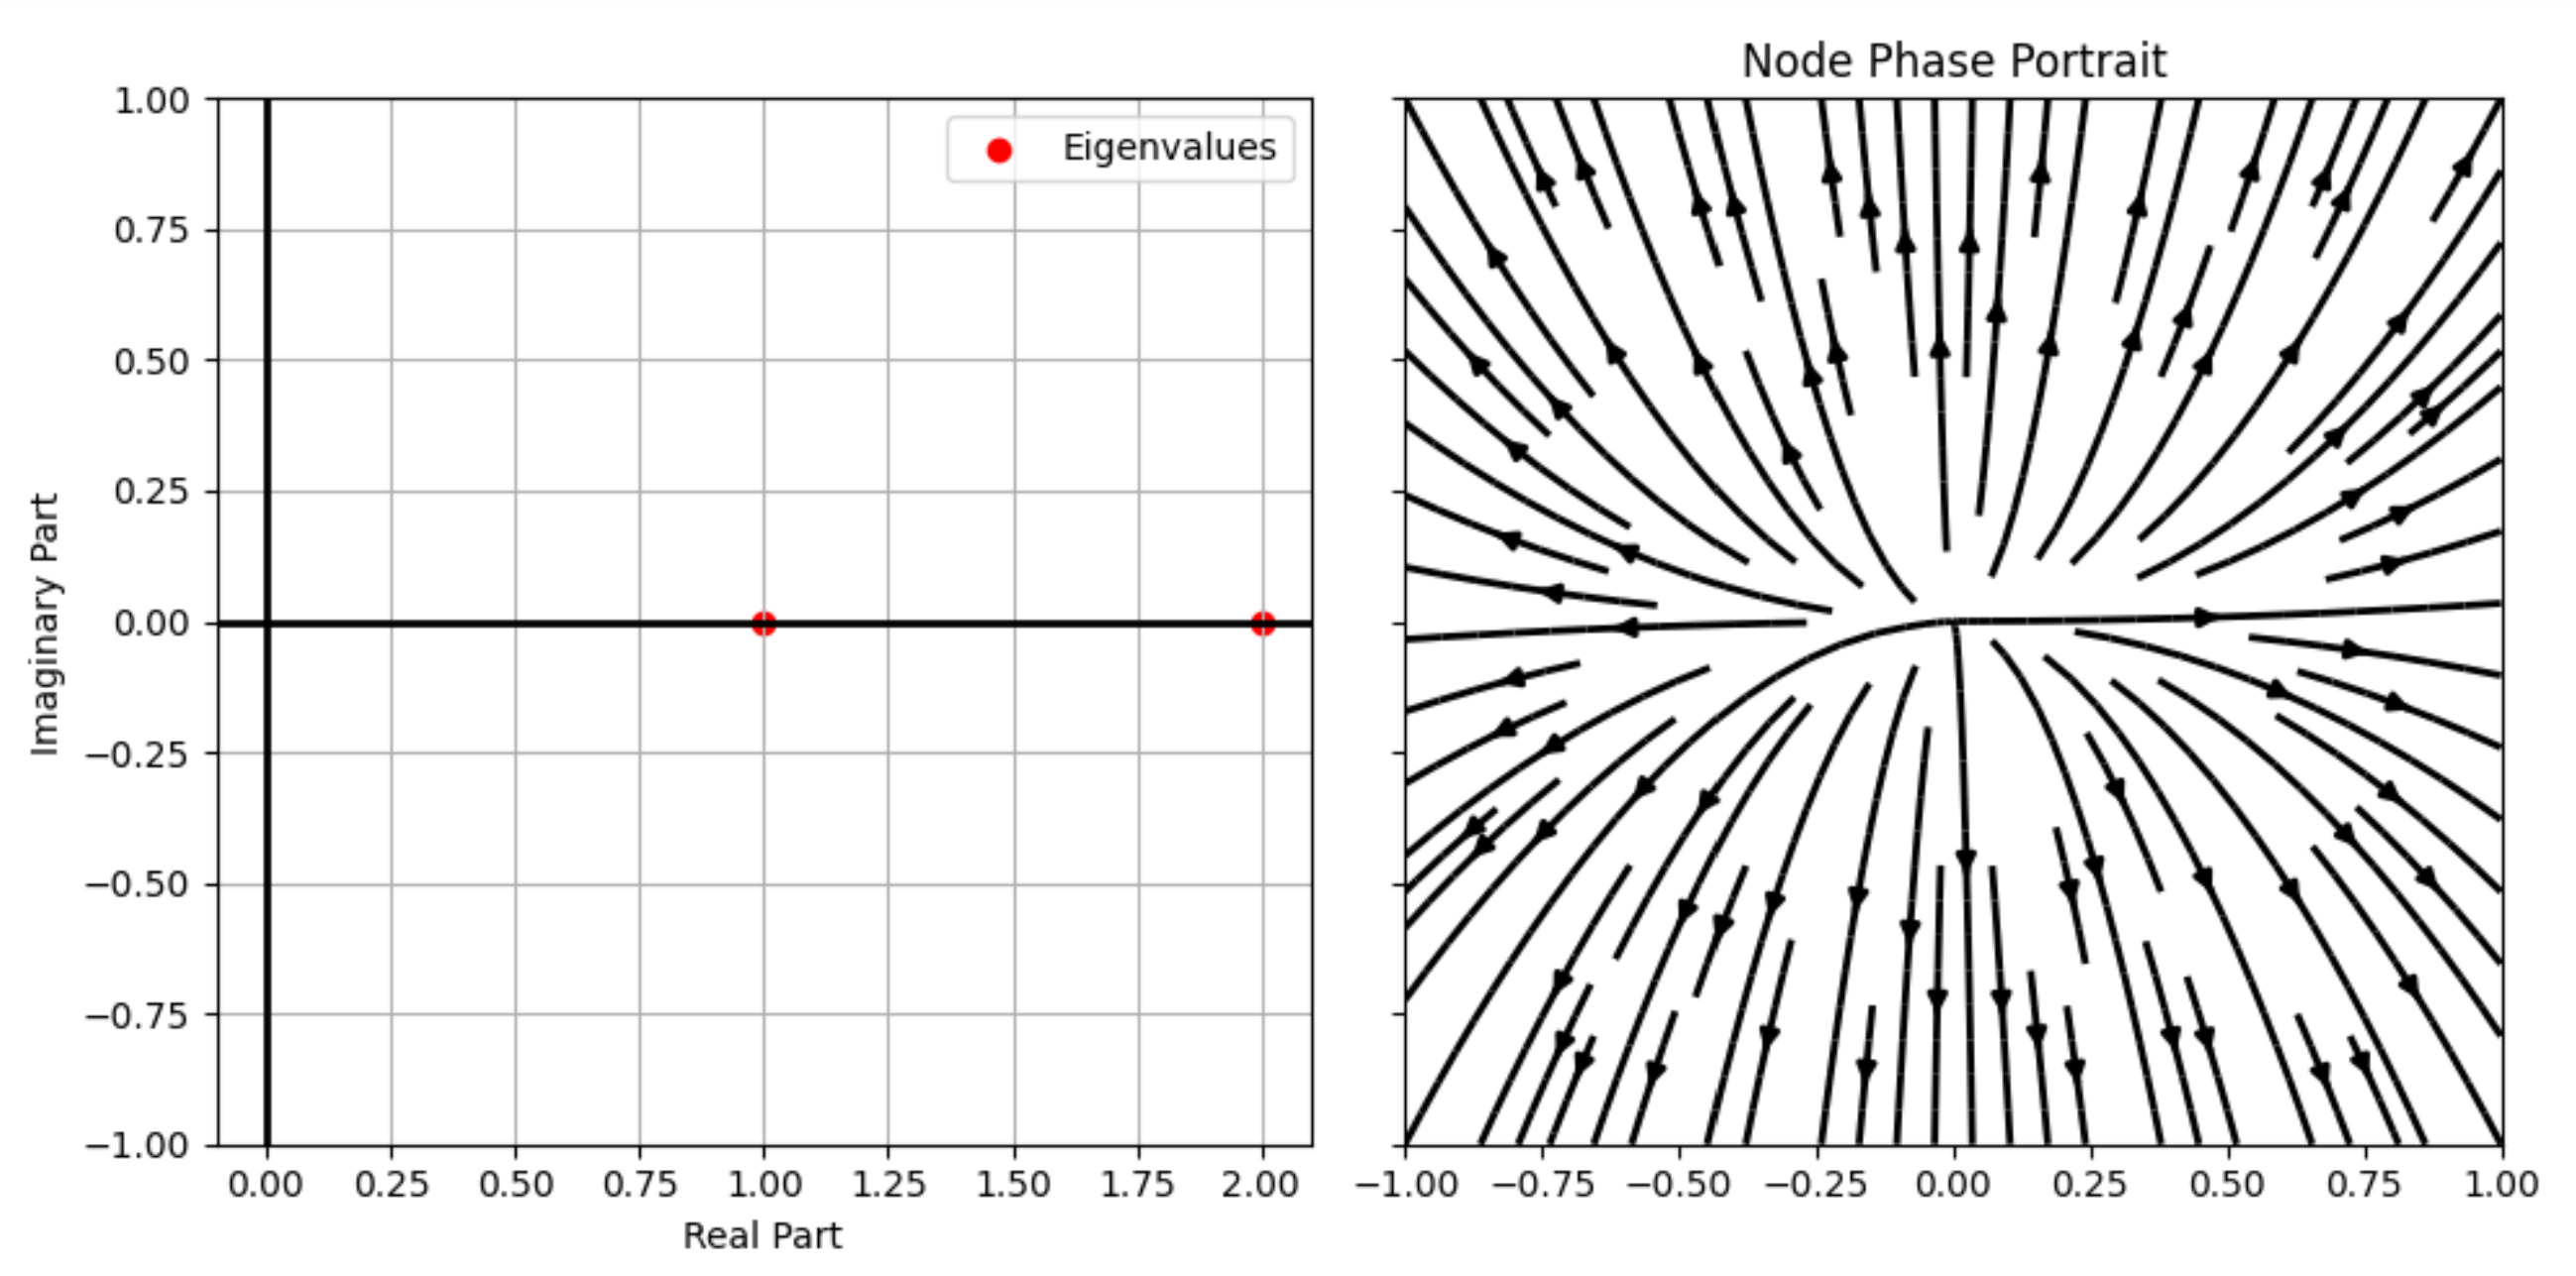
\includegraphics[width=0.8\textwidth]{images/4-1-Node-unstable.png}
    \end{subfigure}
    \begin{subfigure}[b]{\textwidth}
        \centering
        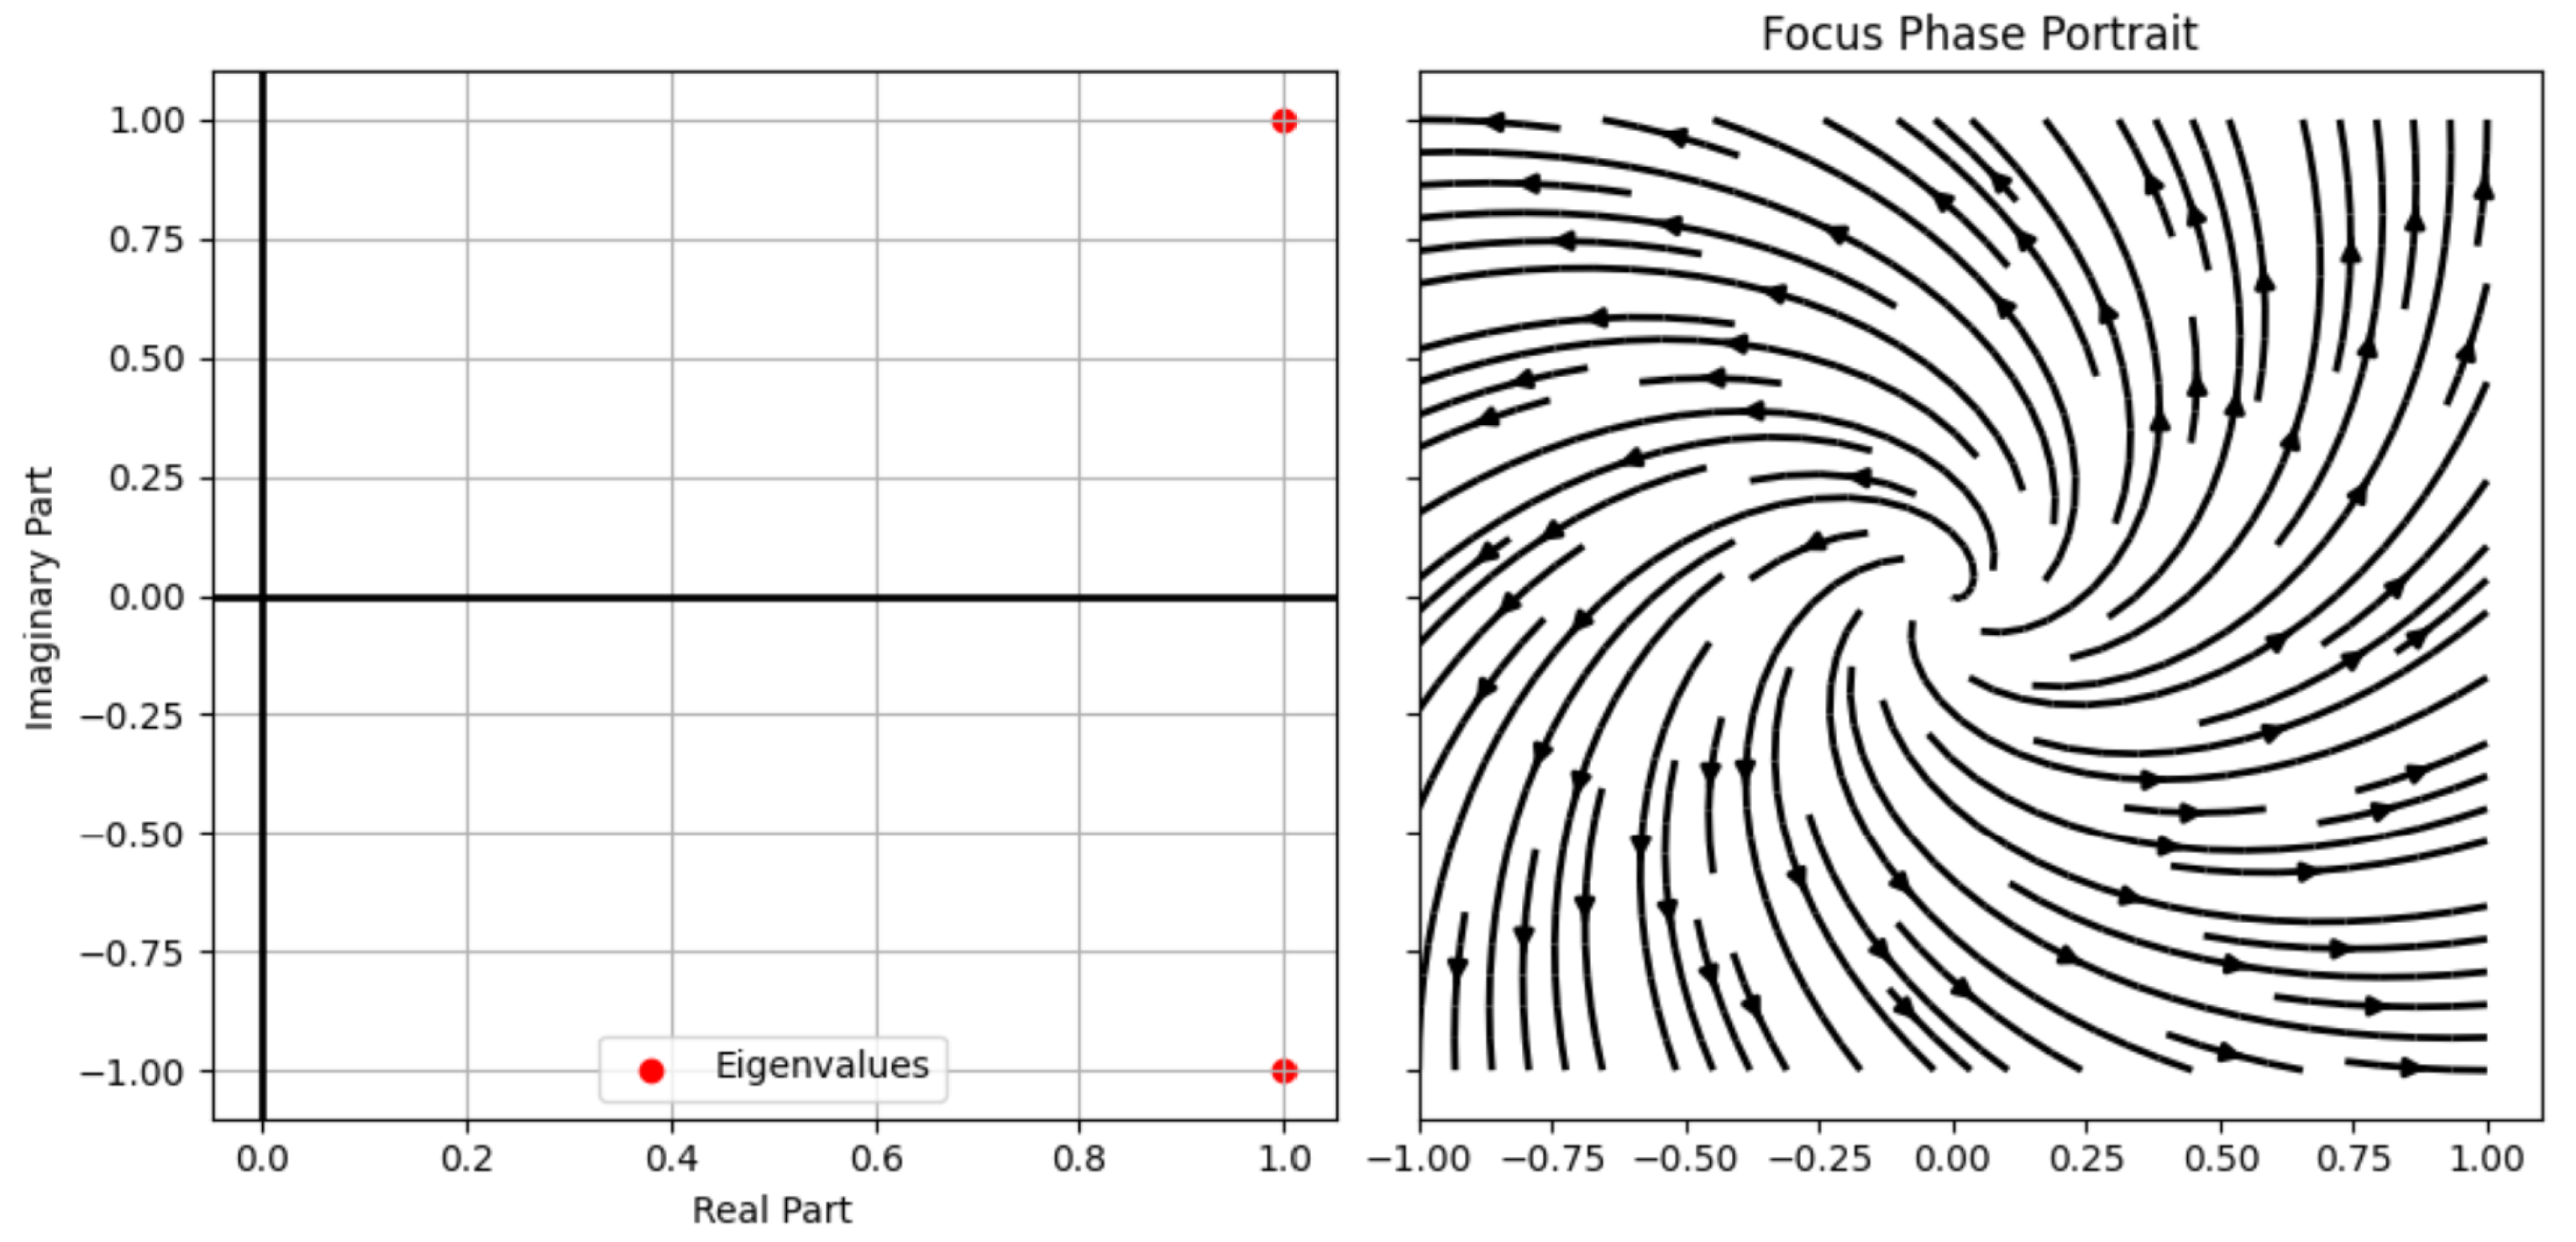
\includegraphics[width=0.8\textwidth]{images/4-1-Focus-unstable.png}
    \end{subfigure}
    \caption{Phase portraits depending on the eigenvalues of the parametrized matrix}
    \label{fig:task1a}
\end{figure}

The first task of exercise 4 asks to construct a figure similar to Fig. 2.5 in the book of Kuznetsov \cite{kuznetsov}. The figure shows a connection between eigenvalues and their corresponding phase portraits. To plot the phase portraits, we utilised the \texttt{streamplot} functionality of \texttt{matplotlib} \cite{Hunter:2007}. \\

% Specify the value of the parameter for each of your phase portraits (ideally in the figure itself).

The following matrices were used (table \ref{tab:task1}): 

\begin{table}[H]
\centering
\begin{tabular}{|l|c|l|}
\hline
\rowcolor[HTML]{FFFFC7} 
\textbf{Eigenvalues}           & \textbf{Matrix} & \textbf{Phase Portrait} \\ \hline

2 real negative                & 
$\begin{bmatrix}
-1 & 0 \\
0 & -2 
\end{bmatrix}$
& Node (stable)           \\ \hline

conjugate complex negative     &
$\begin{bmatrix}
-1 & 1 \\
-1 & -1 
\end{bmatrix}$
& Focus (stable)          \\ \hline

2 real: 1 positive, 1 negative &
$\begin{bmatrix}
+1 & 0 \\
0 & -1 
\end{bmatrix}$
& Saddle (unstable)       \\ \hline

2 real positive                &
$\begin{bmatrix}
+1 & 0 \\
0 & +2 
\end{bmatrix}$
& Node (unstable)         \\ \hline

conjugate complex positive     &
$\begin{bmatrix}
+1 & -1 \\
+1 & +1 
\end{bmatrix}$
& Focus (unstable)        \\ \hline
\end{tabular}
\caption{Eigenvalues, matrices and their resulting phase portraits}
\label{tab:task1}
\end{table}

The stable portraits can be turned into unstable ones and vice versa by changing all the signs within the matrix. The corresponding phase portraits differ in direction only. 

Besides the phase portraits, the eigenvalues were also plotted. First, they were calculated using the \texttt{eig} function of \texttt{Numpy} \cite{harris2020array} and afterward plotted via the function \texttt{scatter} of \texttt{matplotlib}. The resulting graphics are depicted in figure \ref{fig:task1}. \\

% Are these systems topologically equivalent? Why, or why not (no formal proof necessary)?
These systems are not equivalent orbitally or smoothly. However, the orbits can be mapped onto the ones of the next system using a homeomorphism $h: U \rightarrow U$ which is continuous and invertible. This makes the systems topologically equivalent within $U$. 